\documentclass{standalone}
\usepackage{tikz}
\usepackage{ctex,siunitx}
\usepackage{tkz-euclide}
\usepackage{amsmath}
\usetikzlibrary{patterns, calc}
\usetikzlibrary {decorations.pathmorphing, decorations.pathreplacing, decorations.shapes,}
\begin{document}
\small
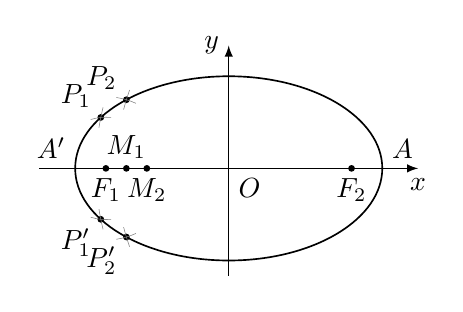
\begin{tikzpicture}[>=latex,scale=0.65]
  \draw[thin,->](-3.7,0)--(3.7,0)node[below]{$x$};
  \draw[thin,->](0,-2.1)--(0,2.4)node[left]{$y$};
  \draw[semithick](0,0)ellipse(3 and 1.8);
  \tkzDefPoints{0/0/O,-2.4/0/F1,2.4/0/F2,-3/0/A',3/0/A,-2.0/0/M1,-1.6/0/M2,-3.4/0/r1,-3.8/0/r2,-2.6/0/R1,-2.2/0/R2}
  \tkzInterCC(F1,r1)(F2,R1)\tkzGetPoints{P1}{P'1}
  \tkzInterCC(F1,r2)(F2,R2)\tkzGetPoints{P2}{P'2}
  % \tkzDrawSegments[densely dashed](M,F1 M,F2)
  \tkzDrawPoints[fill=black](F1,F2,M1,M2,P1,P'1,P2,P'2)
  \tkzCompass[length=0.4](F1,P1)
  \tkzCompass[length=0.4](F2,P1)
  \tkzCompass[length=0.4](F1,P2)
  \tkzCompass[length=0.4](F2,P2)
  \tkzCompass[length=0.4](F1,P'1)
  \tkzCompass[length=0.4](F2,P'1)
  \tkzCompass[length=0.4](F1,P'2)
  \tkzCompass[length=0.4](F2,P'2)
  \tkzLabelPoint[above](M1){$M_1$}
  \tkzLabelPoint[above left](P1){$P_1$}
  \tkzLabelPoint[above left](P2){$P_2$}
  \tkzLabelPoint[below left](P'1){$P'_1$}
  \tkzLabelPoint[below left](P'2){$P'_2$}
  \tkzLabelPoint[below](M2){$M_2$}
  \tkzLabelPoint[below](F1){$F_1$}
  \tkzLabelPoint[below](F2){$F_2$}
  \tkzLabelPoints[above left](A')
  \tkzLabelPoints[above right](A)
  \tkzLabelPoints[below right](O)
\end{tikzpicture}
\end{document}